\AddToHook{package/hyperxmp/before}{\RequirePackage[bookmarksnumbered,unicode]{hyperref}}
\documentclass[sigconf]{acmart}
\settopmatter{printacmref=false, printccs=false, printfolios=true}
\renewcommand\footnotetextcopyrightpermission[1]{}
\setcopyright{none}
\acmConference[ComPar 2026/27]{Computação Paralela -- Projeto 1}{novembro de 2026}{NOVA FCT}
\acmYear{2026}
\acmDOI{}
\acmISBN{}
\usepackage[T1]{fontenc}
\usepackage[portuguese]{babel}
\usepackage{booktabs}
\usepackage{float}
\usepackage{tikz}
\usetikzlibrary{arrows.meta}

% Modelo da UC: quatro páginas de texto/figuras e uma página extra.
% Os resultados são os guardados em experiencias/resultados.
\begin{document}
\title{Análise e otimização de viagens NYC Yellow Taxi com Spark}
\author{Frederico Mestre (77940)}
\email{p177873@campus.fct.unl.pt}
\author{Tiago Pinho (77970)}
\email{p213933@campus.fct.unl.pt}
\renewcommand{\shortauthors}{Mestre e Pinho}

\begin{abstract}
Analisámos 24 meses de viagens NYC Yellow Taxi, de 2023 e 2024,
num cluster Spark em Docker. Implementámos limpeza, análise temporal,
estatísticas por zona, deteção de tarifas anómalas e análise de rotas.
O estudo compara cache, estratégias de junção, cálculo por janela ou
agregação e Adaptive Query Execution (AQE). A cache reduziu a mediana
da pipeline de 101,27 para 76,86~s. AQE teve o maior impacto entre as
alternativas testadas; reduzir as partições iniciais de shuffle deu
diferenças pequenas. Três workers tiveram a menor mediana neste PC,
e passar para seis não trouxe um ganho claro.
\end{abstract}
\keywords{PySpark, NYC Yellow Taxi, profiling, shuffle, Docker}
\maketitle

\section{Introdução}
Usámos os ficheiros mensais Yellow Taxi de 2023 e 2024, publicados
em Parquet pela NYC TLC, e a tabela de zonas~\cite{tlc}. São
79\,479\,946 viagens antes da limpeza e 70\,353\,039 depois dela.
Trabalhar com dois anos permite observar a passagem de dezembro
para janeiro nas janelas temporais, mantendo um volume que conseguimos
medir várias vezes no mesmo computador.

Além de M1--M3, escolhemos O1 e O2~\cite{assignment}. O1 permite
comparar uma janela sobre as viagens com uma agregação seguida de
junção. O2 combina agregações mensais, janelas e duas junções à
tabela de zonas. Assim, conseguimos estudar redistribuição de dados
e reutilização de resultados, em vez de apenas comparar tempos finais.
O objetivo foi perceber que escolhas compensam neste conjunto de
dados e neste ambiente, sem assumir que uma opção é sempre melhor.

\section{Pipeline}
Usámos a API de DataFrames e funções nativas do Spark. Ficámos próximos
dos comandos trabalhados nas Labs e mantivemos os cálculos em
\texttt{projeto1.py}; os notebooks importam essas funções para os
conferir. Não há UDF Python no tratamento das viagens.

\subsection{Leitura e limpeza (M1)}
O schema define os nomes e tipos das colunas, não as partições.
Selecionamos oito colunas e lemos cada mês separadamente, porque
a mesma coluna pode ter tipos físicos diferentes entre ficheiros.
Com \texttt{try\_cast}, convertemos para tipos comuns; valores que
não podem ser convertidos ficam nulos e entram nas contagens de M1.
Depois, \texttt{unionByName} junta as linhas dos meses alinhando as
colunas pelo nome, sem fazer uma junção por chave. Antes de filtrar, marcamos nulos/NaN, tarifa ou distância
não positivas, passageiros fora de 1--6, chegada anterior ou igual à
partida e identificadores de zona fora de 1--263. Acrescentámos um
critério separado para pickups fora do ano do ficheiro.

Uma viagem pode falhar várias regras: as contagens por critério não
se somam para obter o total removido. A Tabela~\ref{tab:limpeza}
apresenta os valores de M1. Guardámos a distância original em milhas
e criámos uma coluna em km, multiplicando por 1,609344. As tarifas
continuam em USD. O fuso da sessão é UTC para tratar as datas sem
fuso da origem de forma independente do fuso do PC.

\begin{table}[t]
\centering
\caption{M1 a 100\%: problemas por ano. Os critérios sobrepõem-se.}
\label{tab:limpeza}
\begin{tabular}{lrr}
\toprule
Critério/contagem & 2023 & 2024 \\
\midrule
Entrada & 38\,310\,226 & 41\,169\,720 \\
Nulos ou NaN & 1\,309\,356 & 4\,091\,232 \\
Tarifa & 394\,503 & 748\,284 \\
Distância & 773\,457 & 776\,305 \\
Passageiros & 583\,414 & 401\,638 \\
Ordem dos timestamps & 15\,569 & 13\,510 \\
Zona & 633\,591 & 425\,660 \\
Ano do pickup & 104 & 56 \\
Removidas, sem duplicar & 3\,231\,939 & 5\,894\,968 \\
Viagens válidas & 35\,078\,287 & 35\,274\,752 \\
\bottomrule
\end{tabular}
\end{table}

\subsection{Análises obrigatórias (M2 e M3)}
M2 junta o borough de partida e agrega por borough, dia da semana e
hora: conta viagens e calcula tarifa, duração em minutos e distância
médias. Escreve Parquet particionado por borough. M3 agrega por zona,
ano e mês, calcula médias e desvios-padrão amostrais e completa a
grelha de 263 zonas por 24 meses, com zero viagens nos meses vazios.
O ranking usa \texttt{dense\_rank}, preservando empates. A quota
móvel usa o mês atual e os dois anteriores. A referência da anomalia
usa os três meses anteriores, sem incluir o mês que estamos a testar;
sem histórico completo, a classificação fica nula.

\subsection{Tarifas e rotas (O1 e O2)}
O1 calcula a média e o desvio-padrão da tarifa por km em cada grupo
(zona de partida, hora). Sinaliza valores superiores a
$\mu+3\sigma$ e compara taxas por borough, pagamento e dia útil/fim
de semana. Em O2 contamos viagens por rota e mês, juntamos os nomes
das duas zonas e calculamos a quota nas partidas da origem. O top-20
de cada borough usa o total do período, com desempate pelos IDs.
Definimos inversão por ano como sinais opostos de
$(s_{mar}-s_{jan})$ e $(s_{set}-s_{jul})$; meses sem viagens da rota
entram com quota zero. Estas regras temporais são convenções do grupo.

Escolhemos O1 para estudar o custo de organizar milhões de viagens
por zona/hora, comparando janelas com estatísticas agregadas e
broadcast. O2 permite estudar a redistribuição por rota e as duas
junções às zonas. Um resultado mensal pequeno não implica pouco
trabalho: a agregação inicial continua a percorrer as viagens.

\begin{figure}[t]
\centering
\begin{tikzpicture}[>=Stealth,every node/.style={font=\scriptsize},
 box/.style={draw,rounded corners=1pt,align=center,inner sep=4pt}]
\node[box] (trips) at (-1.9,0) {Viagens limpas\\InMemoryTableScan};
\node[box] (zones) at (1.9,0) {Zonas\\BroadcastExchange};
\node[box] (join) at (0,-0.85) {BroadcastHashJoin (BuildRight)};
\node[box] (partial) at (0,-1.55) {HashAggregate parcial};
\node[box] (exchange) at (0,-2.25) {Exchange por borough/dia/hora};
\node[box] (final) at (0,-2.95) {AQEShuffleRead coalesced\\HashAggregate final};
\draw[->] (trips) -- (join); \draw[->] (zones) -- (join);
\draw[->] (join) -- (partial); \draw[->] (partial) -- (exchange);
\draw[->] (exchange) -- (final);
\end{tikzpicture}
\caption{Plano simplificado de M2 com broadcast e AQE. A junção evita
redistribuir as viagens por zona, mas a agregação ainda exige shuffle.
Origem: plano final de M2 após \texttt{collect()}, numa inspeção
separada; não é o plano final da escrita da pipeline inteira.}
\Description{Consulta M2: viagens limpas em cache e zonas em broadcast alimentam uma junção hash, agregação parcial, exchange e agregação final com leitura adaptativa coalescida.}
\label{fig:plano}
\end{figure}

\section{Profiling e baseline}
\subsection{Ambiente e método}
As medições correram num PC com Intel Core Ultra 9 275HX, 24 cores
lógicos e cerca de 31,4~GiB de RAM, com Windows 11 e Docker Desktop.
O Docker dispunha de cerca de 15,3~GiB. Usámos Spark 4.2.0 e Python
3.10.12. A configuração principal tem três workers, cada um com
dois cores e 2~GiB anunciados ao Spark, e 1536~MiB por executor.
São seis slots Spark no mesmo PC; não são três máquinas independentes
nem seis cores físicos reservados por quotas Docker.
Escolhemos o cluster Docker por seguir as Labs e satisfazer o mínimo
de cluster pedido no enunciado. Docker também usa os cores do PC;
a alternativa seria \texttt{local[*]}, sem workers distribuídos por
contentores. Não testámos se Docker é mais rápido que esse modo.

Cada configuração teve três corridas, em aplicações Spark novas e
pastas de saída diferentes. Apresentamos a mediana e conservamos
os tempos individuais nos notebooks. O tempo global vai da leitura
até à última escrita, incluindo preencher a cache e guardar os CSV.
Exclui o arranque do Spark e a recolha/exportação das métricas.
Não é a soma dos tempos parciais. Usámos o profiler da Lab~3~\cite{lab3},
que agrega métricas dos stages do bloco. Os tempos acumulados dos
executors não são tempos de parede, e os bytes de entrada podem
incluir leituras da cache, não apenas I/O físico.

Mantivemos os mesmos 24 ficheiros e alterámos uma opção de cada vez.
Nos testes principais usamos 200 partições iniciais de shuffle,
AQE ligado e broadcast das zonas. A opção que força merge só afeta
as zonas; O1 por groupBy continua a usar broadcast das estatísticas.
O README inclui os comandos \texttt{spark-submit}, versões e
configurações; os resultados pequenos e os planos estão no repositório.

\subsection{Referência inicial e verificações}
A baseline completa é a execução sem cache, já com AQE, broadcast
das zonas e O1 por groupBy. Os tempos foram 101,269, 103,528 e
100,620~s: mediana 101,269~s. As medianas de shuffle lido/escrito
foram 129,9/113,2~MiB e o número de tarefas foi 4461. Não registámos
spill de execução nesta referência. Isto não demonstra, por si só,
que não havia custos de memória ou leitura repetida.

As viagens limpas alimentam vários módulos, o que motivou o teste de
cache. Depois, usámos a configuração com cache como referência
comum para O1, joins, AQE e partições. A implementação inicial já
continha várias destas escolhas: os testes com alternativas servem
para as avaliar e justificar a sua manutenção. Não representam
uma sequência de melhorias acumuladas sobre versões diferentes.
Os planos guardados foram inspecionados depois das medições e ajudam
a explicar as diferenças; não foram recolhidos como planos finais
de todas as escritas medidas.

Validámos M1--O2 a 10\% e a 100\%, incluindo contagens, exemplos
diretos, chaves, quotas, rankings e escrita/leitura. Nas comparações
de desempenho conferimos as sete tabelas de saída por chaves.
Contagens e valores discretos têm de coincidir; floats não
arredondados usam tolerância absoluta $10^{-9}$ e relativa $10^{-12}$.
Os testes de arredondamento levaram a usar decimal na tarifa média
de M2/M3 e segundos em decimal na duração média de M2. Estas foram
correções de estabilidade, não otimizações de tempo.

\section{Estudo das otimizações}
Organizamos cada teste em problema observado, hipótese, alteração
isolada e resultado. Esta comparação por ablação desliga uma opção
da referência; não soma ganhos nem pressupõe que todos os mecanismos
já estivessem errados na implementação inicial.

\subsection{Reutilização das viagens limpas}
A hipótese foi que guardar as viagens limpas evitaria repetir a
leitura e a limpeza nos módulos seguintes. Mantivemos as outras
opções e alterámos apenas a cache. Os tempos com cache foram
74,981, 76,861 e 79,109~s. A mediana desceu 24,1\%, contando também
o custo de preencher a cache. As saídas coincidiram com a referência.
Por isso mantivemos cache no DataFrame limpo, libertando-a no fim.
Não concluímos que compensa guardar qualquer DataFrame: aqui há
reutilização suficiente para pagar a materialização.

\subsection{O1: janela ou agregação seguida de junção}
Uma janela coloca as viagens do mesmo grupo juntas e calcula as
estatísticas nesse conjunto. A alternativa agrega primeiro por zona
e hora e distribui a pequena tabela de médias/desvios por broadcast.
A hipótese foi reduzir o volume que passa por ordenação e shuffle.
A mediana de O1 foi 12,68~s com janela e 5,20~s com groupBy;
na pipeline completa, 83,298 e 76,861~s, respetivamente.

As métricas globais ajudam a explicar o resultado: o shuffle escrito
mediano foi 955,4~MiB com janela, contra 129,8~MiB com groupBy;
o spill em disco passou de cerca de 660,8~MiB para zero.
As classificações e os resultados comparados coincidiram.
Mantivemos groupBy, distinguindo o ganho do bloco O1, cerca de
59\%, do ganho global de 7,7\%.

\subsection{Junções com a tabela de zonas}
A tabela de zonas tem apenas 265 linhas. A hipótese foi que copiá-la
para os executors evitaria o shuffle das viagens que uma junção
sort-merge exige. Forçámos a alternativa com \texttt{hint("merge")}
nas junções às zonas, mantendo tudo o resto. Os planos iniciais
mostram \texttt{SortMergeJoin}, ordenações e \texttt{Exchange} nessa
variante; com broadcast mostram \texttt{BroadcastHashJoin}.

A mediana da pipeline foi 95,893~s com merge e 76,861~s com
broadcast, menos 19,8\%. O shuffle escrito mediano foi
4437,4 contra 129,8~MiB, e o spill em disco 3307,5 contra zero.
São métricas da pipeline inteira, não apenas do join.
A Figura~\ref{fig:plano} também mostra o limite da escolha:
broadcast não elimina o shuffle necessário para as agregações.

\subsection{AQE e número inicial de partições}
Com AQE desligado, a mediana subiu para 333,595~s e as tarefas
para 8428, contra 5469 na referência com AQE. Em M2, a mediana
da agregação/escrita foi 144,41~s, e a primeira corrida escreveu
684 ficheiros Parquet, contra 18 com AQE. Agendar tarefas e criar ficheiros tem custos fixos, mesmo com pouco
conteúdo por saída. A hipótese de excesso de pequenas tarefas e
ficheiros é compatível com estes resultados, sem medir o peso de
cada custo separadamente.
Numa inspeção separada, o plano final de M2 apresenta
\texttt{AQEShuffleRead coalesced} com AQE e não o apresenta sem AQE.
Isto apoia a explicação, mas não permite atribuir todo o ganho a
um único mecanismo adaptativo. Mantivemos AQE ligado, incluindo as
opções de coalescência, skew join e leitor local de shuffle.

Testámos ainda 12 e 24 partições iniciais contra as 200 da referência.
Com seis slots, correspondem a duas e quatro partições por slot.
As medianas foram 75,708, 76,223 e 76,861~s. A vantagem observada
de 12 foi só 1,5\%, com intervalos de tempos sobrepostos e uma
referência de 200 medida noutro momento. Na consulta M2 inspecionada,
AQE reduziu os resultados a 2, 2 e 3 partições, respetivamente.
Mantivemos 200: não demonstrámos uma vantagem estável de reduzir
esse valor. São partições iniciais de shuffle, não uma divisão
manual dos ficheiros de entrada com \texttt{repartition}.

\begin{table}[t]
\centering
\caption{Comparações globais. Cada linha mantém as restantes opções;
as reduções não se somam. Tempos em segundos.}
\label{tab:otimizacoes}
\begin{tabular}{lrrr}
\toprule
Alternativa $\rightarrow$ escolha & Antes & Escolha & Redução \\
\midrule
Sem cache $\rightarrow$ cache & 101,27 & 76,86 & 24,1\% \\
O1 janela $\rightarrow$ groupBy & 83,30 & 76,86 & 7,7\% \\
Zonas merge $\rightarrow$ broadcast & 95,89 & 76,86 & 19,8\% \\
AQE desligado $\rightarrow$ ligado & 333,60 & 76,86 & 77,0\% \\
\bottomrule
\end{tabular}
\end{table}

\begin{figure}[t]
\centering
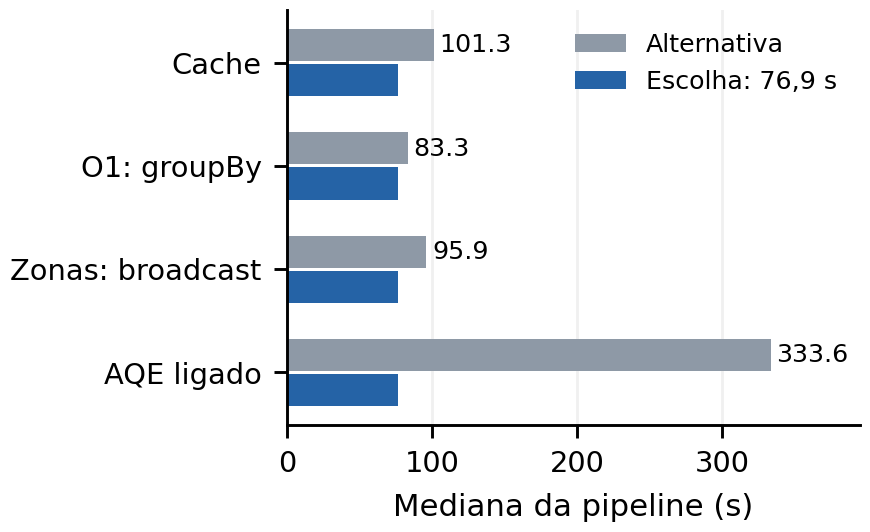
\includegraphics[width=\linewidth]{otimizacoes_relatorio.png}
\caption{Tempos globais das alternativas. A mesma referência com
cache é reutilizada nas comparações, não medida de novo por linha.}
\Description{Quatro comparações de tempo global: sem cache 101,27 segundos; O1 por janela 83,30; zonas por merge 95,89; AQE desligado 333,60. A referência escolhida tem 76,86 segundos.}
\label{fig:otimizacoes}
\end{figure}

\subsection{Complemento local: a mesma pipeline sem Docker}
Repetimos as alternativas num segundo PC sem Docker (\texttt{local[*]},
Windows~11, 16 threads, 8~GB para o driver), com 10\% dos dados, uma ou duas
corridas por configuração e a mesma referência. Os tempos absolutos não são
comparáveis com os do Docker; comparamos só a direção dos efeitos
(Tabela~\ref{tab:local}). Cache e AQE ajudaram nos dois ambientes; o
broadcast valeu menos em local, onde o shuffle não sai do processo, e no O1
janela e groupBy empataram (13,1 e 13,7~s).

A maior diferença foi nas partições (Figura~\ref{fig:particoes}): em local,
200~$\to$~32 reduziu a pipeline de 163 para 59~s, com 8 a 32 partições
equivalentes e 64 já pior, e de 211 para 109~s com todos os dados. A nossa
hipótese, não verificada, é um custo fixo maior por tarefa e por ficheiro em
Windows (por exemplo, as chamadas ao \texttt{winutils}), que a coalescência do
AQE não compensa. A melhor escolha para esta opção depende, assim, do
ambiente de execução.

\begin{table}[H]
\centering
\caption{Redução do tempo da pipeline com cada escolha, nos dois ambientes.}
\label{tab:local}
\begin{tabular}{lrr}
\toprule
Alternativa $\rightarrow$ escolha & Local & Docker \\
\midrule
Sem cache $\rightarrow$ cache & 17\% & 24,1\% \\
Zonas merge $\rightarrow$ broadcast & 8\% & 19,8\% \\
AQE desligado $\rightarrow$ ligado & 61\% & 77,0\% \\
O1 janela $\rightarrow$ groupBy & n.s. & 7,7\% \\
200 partições $\rightarrow$ 32 / 12 & 64\% & 1,5\% \\
\bottomrule
\end{tabular}
\end{table}

\begin{figure}[H]
\centering
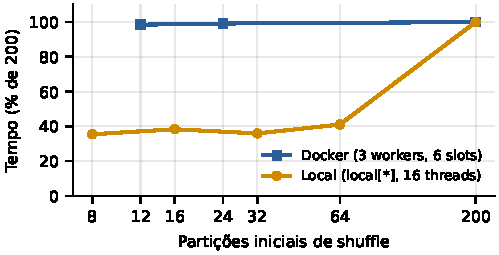
\includegraphics[width=\linewidth]{particoes_relatorio.pdf}
\caption{Tempo da pipeline em função das partições iniciais de shuffle,
em percentagem do tempo com 200 em cada ambiente. Os tempos absolutos
não são comparáveis entre ambientes.}
\Description{Em Docker, 12, 24 e 200 partições dão tempos praticamente iguais. Em local, 8 a 64 partições ficam entre 35 e 41 por cento do tempo com 200.}
\label{fig:particoes}
\end{figure}


\section{Análise de escalabilidade}
Usámos a configuração escolhida: cache, broadcast das zonas, O1 por
groupBy, AQE e 200 partições iniciais de shuffle. As experiências de
escala têm aplicações novas e três repetições próprias. A referência
de três workers passou a ter mediana 76,546~s; não substituímos os
76,861~s das experiências anteriores.

\subsection{Amostra de 10\% e conjunto completo}
A amostra usa seed 42 depois de unir os 24 ficheiros. Conserva
7\,947\,434 viagens antes da limpeza e 7\,036\,182 depois. Os
tempos foram 46,842, 44,523 e 45,802~s, com mediana 45,802~s.
Com todos os dados, a mediana foi 76,546~s
(Figura~\ref{fig:amostra}). Cerca de dez vezes mais viagens válidas
exigiram 1,67 vezes o tempo: crescimento sublinear observado.

A amostra continua a percorrer os mesmos ficheiros; não representa
ler só 10\% dos bytes físicos. Há custos fixos de planeamento,
agendamento e escrita, e M3 mantém as 6312 linhas da grelha zona/mês.
Isto ajuda a interpretar o resultado, sem demonstrar uma lei geral
de escala. Como complemento, um, dois e três anos tiveram medianas
45,932, 76,546 e 101,328~s. O caso de três anos acrescenta 2022;
não substitui a comparação de amostragem e muda o histórico de M3.

\begin{figure}[t]
\centering
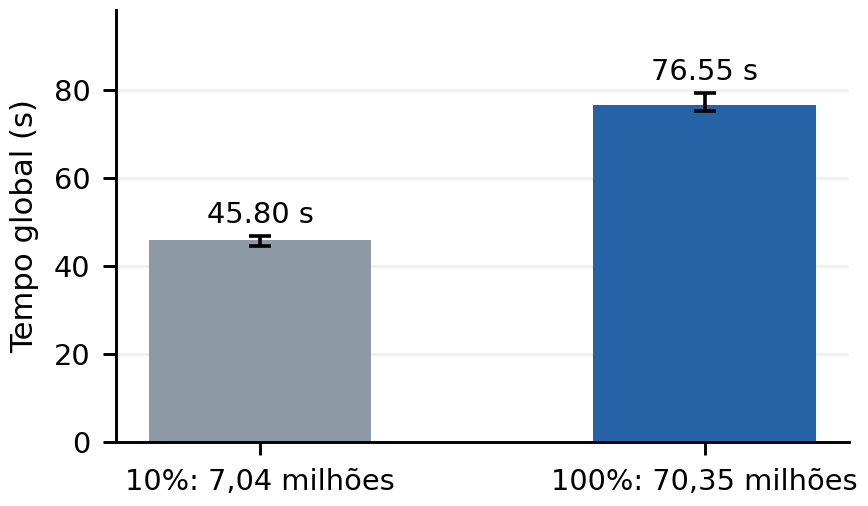
\includegraphics[width=\linewidth]{amostra_relatorio.png}
\caption{Pipeline com 10\% e 100\%, três workers. Barras de erro:
mínimo e máximo das três corridas, não intervalos de confiança.}
\Description{Tempo mediano de 45,80 segundos com amostra de dez por cento e 76,55 segundos com dados completos, em três workers.}
\label{fig:amostra}
\end{figure}

\subsection{Número de workers}
Repetimos os dados completos com 1, 2, 3 e 6 workers, em três rondas
nessa ordem. Calculámos $S_N=T_1/T_N$ e $E_N=S_N/N$; a referência
tem um worker de dois slots, não execução sequencial num core.
A Tabela~\ref{tab:escala} e a Figura~\ref{fig:workers} mostram os
resultados. De dois para três workers, o speedup foi 1,27 para um
aumento de recursos de 1,5 vezes, ou cerca de 84,4\% de eficiência
relativa a dois workers.

\begin{table}[t]
\centering
\caption{Escala com dados fixos; mediana de três corridas.}
\label{tab:escala}
\begin{tabular}{rrrrr}
\toprule
Workers & Slots & Tempo (s) & $S_N$ & $E_N$ \\
\midrule
1 & 2 & 137,38 & 1,00 & 100,0\% \\
2 & 4 & 96,85 & 1,42 & 70,9\% \\
3 & 6 & 76,55 & 1,79 & 59,8\% \\
6 & 12 & 77,65 & 1,77 & 29,5\% \\
\bottomrule
\end{tabular}
\end{table}

\begin{figure}[t]
\centering
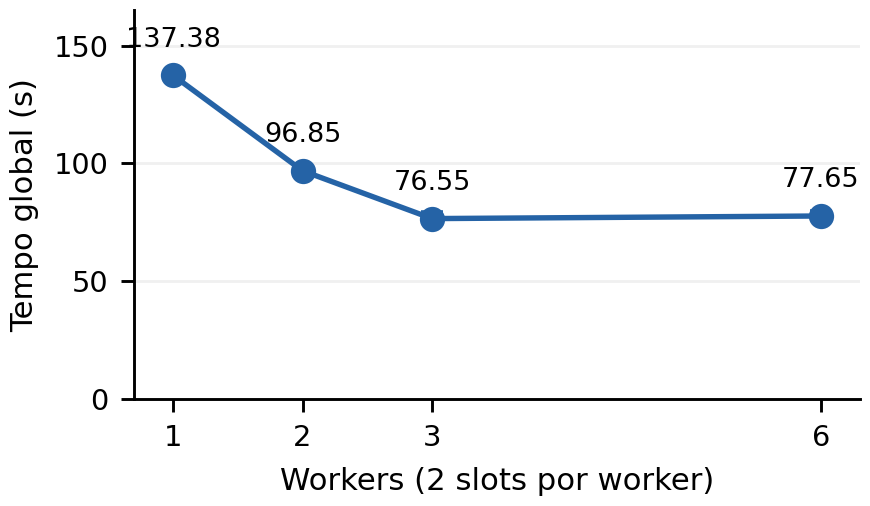
\includegraphics[width=\linewidth]{workers_relatorio.png}
\caption{Tempo com 1, 2, 3 e 6 workers no mesmo PC. Barras de erro:
mínimo e máximo de três corridas.}
\Description{Tempos medianos para um, dois, três e seis workers: 137,38; 96,85; 76,55; 77,65 segundos.}
\label{fig:workers}
\end{figure}

Três workers deram a menor mediana. Seis tiveram 77,653~s e tempos
sobrepostos aos de três, sem vantagem clara. Mais workers partilham
o mesmo disco e processador, acrescentam coordenação e aumentam
também a memória total anunciada ao Spark. A experiência não isola
o efeito do número de cores nem reproduz uma escala em máquinas
independentes. Mantivemos três workers como escolha prática para
este PC, sem afirmar que é o ótimo em qualquer cluster.

\section{Discussão}
O maior contraste observado foi AQE ligado/desligado. A escrita
de M2 mostrou que o número de pequenas tarefas e ficheiros pode
pesar mais do que esperávamos. A cache também compensou, porque
os mesmos dados limpos alimentam várias operações. Em sentido
contrário, reduzir as partições iniciais ou duplicar os workers de
três para seis não trouxe uma melhoria suficientemente clara.
Os resultados mostram por que precisamos de medir tempo, shuffle,
spill e tarefas em conjunto: por exemplo, com cache houve mais
tarefas do que na baseline, mas menos tempo global.

Há limitações. Só fizemos três repetições, a ordem não foi
aleatória e não controlámos a cache de ficheiros do sistema
operativo nem toda a atividade do PC. Nas partições, alternámos
12/24, mas reutilizámos as corridas anteriores de 200. Não medimos
distribuições de duração de tarefas para diagnosticar skew, não
há estudo de UDF e não testámos outras ordens de múltiplos joins.
Os planos separados ajudam a interpretar os operadores, mas não
provam qual foi o peso de cada operador nas escritas medidas.

Com mais tempo, repetiríamos as alternativas próximas em ordem
alternada, recolheríamos métricas por tarefa e testaríamos noutro
computador ou cluster com nós independentes. Também fixaríamos as
dependências e a imagem Docker por versão imutável: o README
regista as versões observadas, mas um build futuro pode mudar.
A conclusão atual é limitada aos dados, recursos e opções testados;
preservar os resultados foi condição para aceitar cada escolha.

\clearpage
\begin{thebibliography}{3}
\bibitem{assignment}
Hervé Paulino. 2026. \textit{ComPar 26/27 Project Assignment 1:
Large-Scale Analytics with Spark}. Enunciado da unidade curricular.
\bibitem{tlc}
NYC Taxi and Limousine Commission. \textit{TLC Trip Record Data}.
Dados Yellow Taxi de 2023 e 2024 e Taxi Zone Lookup Table.
\url{https://www.nyc.gov/site/tlc/about/tlc-trip-record-data.page}.
URLs mensais e hashes em \texttt{download\_manifest.csv} no repositório.
\bibitem{lab3}
Computação Paralela. 2026. \textit{Lab 03: Spark Profiling and
Optimization}. Notebooks e helper \texttt{spark\_profiler.py}
fornecidos nos materiais da unidade curricular.
\end{thebibliography}

\section*{Agradecimentos e utilização de IA}
Agradecemos os materiais das aulas e das Labs, que serviram de base
à implementação e ao estudo de desempenho, incluindo o profiler da Lab~3.

Usámos o ChatGPT/Codex e Claude para esclarecer e rever comandos menos
familiares, apoiar correções numéricas e criar verificações de
resultados. Exemplos: conversões com \texttt{try\_cast}, união com
\texttt{unionByName}, limites de \texttt{rangeBetween}, comparações
com \texttt{exceptAll} e médias em decimal. O apoio incluiu também
preparar e executar experiências, interpretar métricas, organizar
notebooks e preparar o rascunho deste relatório. A base de trabalho partiu dos materiais das aulas e das Labs e foi
desenvolvida por ambos, com o apoio de IA descrito acima.

Os pedidos incluíram, em resumo: investigar diferenças de arredondamento a 10\% e 100\%; medir o
efeito da cache e interpretar as métricas e os planos de execução do Spark. Não desenvolvemos
um agente próprio. O registo de IA documenta os pedidos e alterações;
as regras de trabalho foram preservar dados e resultados, separar
validação de medição e justificar as conclusões com evidência.

\section*{Contribuições individuais}
\textbf{Frederico Mestre (77940) --- 50\%.} Preparação da baseline,
desenvolvimento e testes da pipeline, estudo das alternativas de otimização
e preparação de texto sobre a pipeline e as otimizações.

\textbf{Tiago Pinho (77970) --- 50\%.} Preparação e validação no Docker,
experiências de desempenho e escalabilidade, organização das evidências
e integração do relatório.

Ambos trabalharam sobre a pipeline completa. A escolha do ambiente
final, a discussão dos resultados e as conclusões são trabalho coletivo.
A divisão de 50\% para cada elemento reflete a contribuição global,
não a atribuição exclusiva de módulos a uma pessoa.


% Conferir as declarações e o pacote final antes da entrega.
\end{document}
